%************************************************
\chapter{Motivación e Introducción}\label{ch:introduction}
%************************************************

\todo[inline]{Pipeline Genérico, detallar cada parte, con ejemplos y
  justificación}

\todo[inline]{Pipeline Específico, con paquete real (CoreNLP), explicar de forma
  breve cada parte, inglés)}

\todo[inline]{Desribir de forma más detallada el Dep Parsing, mencionar state of
  the art (3/4 papers), entre ellos el implementado}

\todo[inline]{Sección con algoritmo implementado, reiterando sección anterior
  pero con lujo de detalles (Teóricos y código)}

\todo[inline]{Añadir sección ``\emph{El resto del paper está organizado\dots}''}

\section{¿Qué es el Procesamiento del Lenguaje Natural?}
\label{sec:whatisnlp}

El lenguaje natural se refiere a cualquier lenguaje hablado por un humano, (\eg
Inglés, Castellano o Chino). El \acfi{NLP}\acused{NLP}\graffito{\acf{PNL}} es un
campo de la ciencia de la computación e ingeniería desarrollado a partir del
estudio del lenguaje y la computación lingüistica dentro del campo de la
\ac{IA}. Los objetivos del \ac{NLP} son diseñar y construir aplicaciones que
faciliten la interacción humana con la máquinas y otros dispositivos mediante el
uso del lenguaje natural. Dentro del amplio campo del \ac{NLP} podemos
distinguir las siguientes áreas principales:

El lenguaje natural se refiere a cualquier lenguaje hablado por un humano, (\eg
Inglés, Castellano o Chino). El \ac{NLP}\graffito{\acf{PNL}} es un campo de la
ciencia de la computación e ingeniería desarrollado a partir del estudio del
lenguaje y la computación lingüistica dentro del campo de la \ac{IA}. Los
objetivos del \ac{NLP} son diseñar y construir aplicaciones que faciliten la
interacción humana con la máquinas y otros dispositivos mediante el uso del
lenguaje natural. Dentro del amplio campo del \ac{NLP} podemos distinguir las
siguientes áreas principales:

\paragraph{Resúmenes} este área incluye aplicaciones que puedan, basándose en
una colección de documentos, dar como salida un resumen coherente del contenido
de los mismos. Otra de las posibles aplicaciones sería generar presentaciones a
partir de dichos documentos. En los últimos años, la información disponible en
la red ha aumentado considerablemente. Un claro ejemplo es la literatura
científica, o incluso repositorios de información más genérica como
\emph{Wikipedia}. Toda esta información escrita en lenguaje natural puede
aprovecharse para entrenar modelos que sean capaces de generar hipótesis por sí
mismos, generar resúmenes o extraer hechos. Un ejemplo claro puede ser la
extracción de hechos básicos que relacionen dos entidades (\emph{``Luís es padre
de Cristina''}.

\paragraph{Traducción automática:} Esta fue la principal área de investigación
en el campo del \ac{NLP}. Como claro ejemplo tenemos el traductor de Google,
mejorando día a día. Sin embargo, un traductor realmente útil sería aquel que
consiga traducir en tiempo real una frase que le dictemos mientras decidimos qué
línea de autobús debemos coger para llegar a tiempo a una conferencia en
Zurich. La traducción entre lenguajes es quizá una de las formas más
transcendentales en las que las máquinas podrían ayudar en comunicaciones entre
humanos. Además, la capacidad de las máquinas para traducir entre idiomas
humanos se considera aún como un gran test a la \ac{IA}, ya que una traducción
correcta no consiste en el mero hecho de generar frases en un idioma humano,
también requiere del conocimiento humano y del contexto, pese a las ambigüedades
de cada idioma. Por ejemplo, la traducción literal \emph{``bordel''} en Francés
significa Burdel; pero si alguien dice \emph{``Mi cuarto es un burdel''}, el
traductor debería tener el conocimiento suficiente para inferir que la persona
se está refiriendo a que su habitación es un desorden.

La traducción automática fue una de las primeras aplicaciones no numéricas de la
computación y comenzó a estudiarse de forma intensiva en la década de los
50. Sin embargo, no fue hasta la década de los 90 cuando se produjo una
tansformación en este área. IBM se hizo con una gran cantidad de frases en
Inglés y Francés que eran traducciones las unas de las otras, \graffito{Conocido
como texto paralelo} lo cual permitió recopilar estadísticas de traducciones de
palabras y secuencias de palabras, concediento así el desarrollo de modelos
probabilísticos para la traducción automática. Hasta ese momento, todo el
análisis gramático se hacía manualmente.

A la llegada del nuevo milenio, se produjo una explosión de texto disponible en
la red, así como grandes cantidades de \emph{texto paralelo}. Se dieron
invención a nuevos sistemas para la traducción automática basados en modelos
estadísticos basados en frases en lugar de palabras. En lugar de traducir
palabra por palabra, ahora se tenían en cuenta pequeños grupos de palabras que a
menudo poseen una traducción característica.

En los últimos años, y mediante el uso de \emph{deep learning} se están
desarrollando modelos de secuencias basados en este tipo de aprendizaje bastante
prometedores. La idea principal del \emph{deep learning} reside en entrenar un
modelo con varios niveles de representación para optimizar el objetivo deseado,
una traducción de calidad, en este caso. Mediante estos niveles el modelo puede
aprender representaciones intermedias útiles para la tarea que le ocupa. Este
método de aprendizaje se ha explotado sobre todo en redes neuronales. Un ejemplo
claro de \emph{deep learning} usando redes neuronales es el reconocimiento de
dígitos, cada capa interna de la red neuronal intenta extraer características
representativas de cada dígito a distintas escalas. Podemos ver una demostración
de este comportamiento en \citet{computerPhile:nn}

\paragraph{Reconocimiento de voz:} Una de las tareas más difíciles en
\ac{NLP}. Aún así, se han conseguido grandes avances en la construcción de
modelos que pueden usarse en el teléfono móvil o en el ordenador. Estos modelos
son capaces de reconocer expresiones del lenguaje hablado como preguntas y
comandos. Desafortunadamente, los sistemas
\acfi{ASR}\acused{ASR}\graffito{\acf{RVA}} funcionan bajo dominios muy acotados
y no permiten al interlocutor desviarse de la entrada que espera el sistema, \eg
\emph{``Por favor, diga ahora la opción a elegir: 1 Para\dots, 2 para\dots''}

\paragraph{SDS:} Los \emph{\acp{SDS}}\graffito{\ac{SDS}: Sistemas de Diálogo
  Hablados}. El diálogo ha sido un tema popular para el \ac{NLP} desde los
80. En estos sistemas se pretende remplazar a los usuales buscadores en los que
introducimos un texto para obtener algún tipo de respuesta a una pregunta. Por
ejemplo, si quisieramos saber a qué hora abre un centro comercial, bastaría con
hablarle al sistema en lenguaje natural -- nuestro lenguaje natural, ya sea
Inglés, Alemán o Castellano y el sistema nos daría respuesta a nuestra
pregunta. Aunque ya existen este tipo de sistemas (\eg \emph{Siri de Apple,
  Cortana de Microsoft, Google Now\dots}) están aún en una situación muy
precaria, ya que ninguno entiende por completo el lenguaje natural, solo un
subconjunto de frases clave.

La creación de \acp{SDS}, ya sea entre humanos o entre humanos y agentes
artificiales requiere de herramientas como:
\begin{itemize}
\item \ac{ASR}, para identificar qué dice el humano.
\item \acfi{DM}\acused{DM}\graffito{\ac{DM}: Gestión del diálogo}, para
  determinar qué quiere el humano.
\item Acciones para obtener la información o realizar la actividad
  solicitada.
\item Síntesis \acfi{TTS}\acused{TTS}\graffito{Leer un texto por una
    máquina}, para comunicar dicha información al humano de forma hablada.
\end{itemize} En la actualidad, \citet{microsoft:sds} desarrollaron un \ac{SDS}
haciendo uso de \emph{deep learning} para asociar señales sonoras a secuencias
de palabras y sonidos del idioma humano, logrando avances importantes en la
precisión del reconocimiento del habla.

\paragraph{Clasificación de documentos:} Una de las áreas más exitosas del
\ac{NLP}, cuyo objetivo es identificar a qué categoría debería pertenecer un
documento. Ha demostrado tener un amplio abanico de aplicaciones, \eg filtrado
de \emph{spam}, clasificación de artículos de noticias, valoraciones de
películas\dots Parte de su éxito e impacto se debe a la facilidad relativa que
conlleva entrenar los modelos de aprendizaje para hacer dichas clasificaciones.

\paragraph{Análisis de Sentimientos:} Gran parte del trabajo en \ac{NLP} se ha
centrado en el análisis de sentimientos (identificación de orientaciones
positivas o negativas en textos) e identificación de creencias positivas,
negativas o neutrales en frases basándose en información léxica y
sintáctica. Tanto las creencias como los sentimientos constitiyen actitudes
hacia eventos y proposiciones, aunque en concreto, los sentimientos pueden
también referirse a actitudes hacia objetos tales como personas, organizaciones
y conceptos abstractos. La detección de sentimientos y emociones en texto
requiere de información léxica y a nivel de la propia sentencia. Por lo general,
el sentimiento puede detectarse a través del uso de palabras expresando
orientaciones positivas o negativas, \eg \emph{triste, preocupado, difícil} son
todas palabras con una connotación negativa, mientras que \emph{cómodo,
  importante, interesante} denotan un sentimiento positivo. Las aproxmiaciones
más sofisticadas para el anlálisis de sentimientos intentan buscar tanto la
fuente como el objeto del sentimiento, \eg quién está expresando un sentimiento
positivo sobre alguna persona, objeto, actividad o concepto.

La comunidad del reconocimiento de voz está igualmente implicada en el estudio
de actitudes positivas y negativas, centrándose en la identifiación de emociones
haciendo uso de información acústica y prosódica, es decir un relieve en la
pronunciación. Otras investigaciones se han centrado en identificar emociones
particulares, específicamente las séis emociones básicas según Ekman -- ira,
aversión, temor, dicha, tristeza y asombro -- las cuales pueden ser reacciones a
eventos, proposiciones u objetos. Por contra, la generación de emociones ha
demostrado ser un reto mucho mayor para la síntesis \ac{TTS}.

La clasificación de sentimientos es algo ampliamente usado para identificar
opiniones -- puntos de vista positivos o negativos hacia personas, instituciones
o ideas -- en muchos idiomas y géneros. Una de las aplicaciones más prácticas, y
de las que más abundan consiste en identificar críticas sobre películas o
productos \cite{Pang:2002:TUS:1118693.1118704,Wang2014}.

La minería de datos en redes sociales con el fin de realizar análisis de
sentimientos se ha convertido en un tema popular con el objetivo de evaluar el
\emph{estado de ánimo} del público -- de twitter, por ejemplo. -- 

El \ac{NLP} emplea técnicas computacionales con el propósito de aprender,
entender y producir lenguaje humano. Las aproximaciones de hace unos años en el
campo de la investigación del lenguaje se centraban en automatizar el análisis
de las estructuras lingüísticas y desarrollar tecnologías como las mencionadas
anteriormente. Los investigadores de hoy en día se centran en usar dichas
herramientas en aplicaciones para el mundo real, creando sistemas de diálogo
hablados y motores de traducción \emph{Speech-to-Speech}, es decir, dados dos
interlocutores, interpretar y traducir sus frases. Otro de los focos en los que
se centran las investigaciones actuales son la minería en redes sociales en
busca de información sobre salud, finanzas e identificar los sentimietos y
emociones sobre determinados productos.

\section{Historia del Procesamiento del Lenguaje Natural}
\label{sec:currentnlp}

A continuación, citamos algunos de los avances en este campo durante los últimos
años según \citet{Hirschberg2015}.

Durante las primeras épocas de esta ciencia, se intentaron escribir vocabularios
y reglas del lenguaje humano para que el ordenador las entendiera. Sin embargo,
debido a la naturaleza ambigua, variable e interpretación dependiente del
contexto de nuestro lenguaje resultó una ardua tarea. Por ejemplo, una estrella
puede ser un ente astronómico o una persona, y puede ser un nombre o un verbo.

En la década de los 90, los investigadores transformaron el mundo del \ac{NLP}
desarrollando modelos sobre grandes cantidades de datos sobre lenguajes. Estas
bases de datos se conocen como \emph{corpus}. El uso de estos conjuntos de datos
fueron uno de los primeros éxitos notables del uso del \emph{big data}, mucho
antes de que el \ac{AA} acuñara este término.

Esta aproximación estadística al \ac{NLP} descubrió que el uso de métodos
simples usando palabras, secuencias del
\acfi{POS}\acused{POS}\graffito{\ac{POS}: Categorías morfosintácticas en
  castellano} (si una palabra es un nombre, verbo o preposición), o plantillas
simples pueden obtener buenos resultados cuando son entrenados sobre un gran
conjunto de datos. A día de hoy, muchos sistemas de clasificación de texto y
sentimientos se basan únicamente en los distintos conjuntos de palabras o
\emph{``bag of words''} que contienen los documentos, sin prestar atención a su
estructura o significado. El estado del arte de hoy día usa aproximaciones con
\ac{AA} y un rico conocimiento de la estructura lingüística. Un ejemplo de estos
sistemas es \emph{Stanford \textsc{CoreNLP}} \citep{Manning2014}. \emph{\textsc{CoreNLP}}
proporciona un \emph{pipeline} estándar para el procesamiento del \ac{NLP}
incluyendo:

\paragraph{POS Tagging:}Etiquetado morfosintáctico. Módulo encargado de leer
texto en algún lenguaje y asignar la categoría morfosintáctica a cada palabra,
\eg nombre, verbo, adjetivo\dots aunque por lo general se suelen usar etiquetas
más detalladas como ``\emph{nombre-plural}''.

\paragraph{NER:}\acfi{NER}\acused{NER}, etiqueta palabras en un texto
correspondientes a \emph{nombres de cosas}, como personas, nombres de compañías,
nombres de proteínas o genes etc. En concreto, \emph{\textsc{CoreNLP}} distingue de forma
muy precisa tres tipos de clases, personas, organizaciones y localizaciones.

\paragraph{Parseo Gramatical:}Resuelve la estructura gramatical de frases, \eg
qué grupos de palabras van juntos formando frases y qué palabras son sujeto u
objeto de un verbo. Como se ha comentado, en aproximaciones anteriores se usaban
parseadores probabilísticos usando conocimiento del lenguaje a partir de
sentencias analizadas sintácticamente a mano. Para así producir el análisis más
probable de sentencias nuevas. Actualmente se se usan parseadores estadísticos,
los cuales aún comenten fallos, pero funcionan bien a rasgos generales.

\paragraph{DP:}\acfi{DP}\acused{DP} o parseo de dependencias. Analiza la
estructura gramatical de una frase, estableciendo relaciones entre palabras
principales y palabras que modifican dichas palabras principales. La
\autoref{fig:nndep} muestra un ejemplo. La flecha dirigida de la palabra
\emph{moving} a la palabra \emph{faster} indica que \emph{faster} modifica a
\emph{moving}. La flecha está etiquetada con una palabra, en este caso
\emph{advmod}, indicando la naturaleza de esta dependencia. La
\autoref{fig:corenlp} muestra ejemplos de los distintos módulos del
\emph{pipeline} de \emph{\textsc{CoreNLP}}

\begin{figure}[bth]
  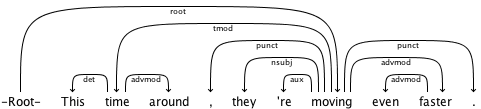
\includegraphics[width=1\linewidth]{gfx/nndep-example}
  \caption[Ejemplo de parseo de dependencias]{Ejemplo de parseo de dependencias}
  \label{fig:nndep}
\end{figure}

\begin{figure}[bth]
\makebox[\textwidth][c]{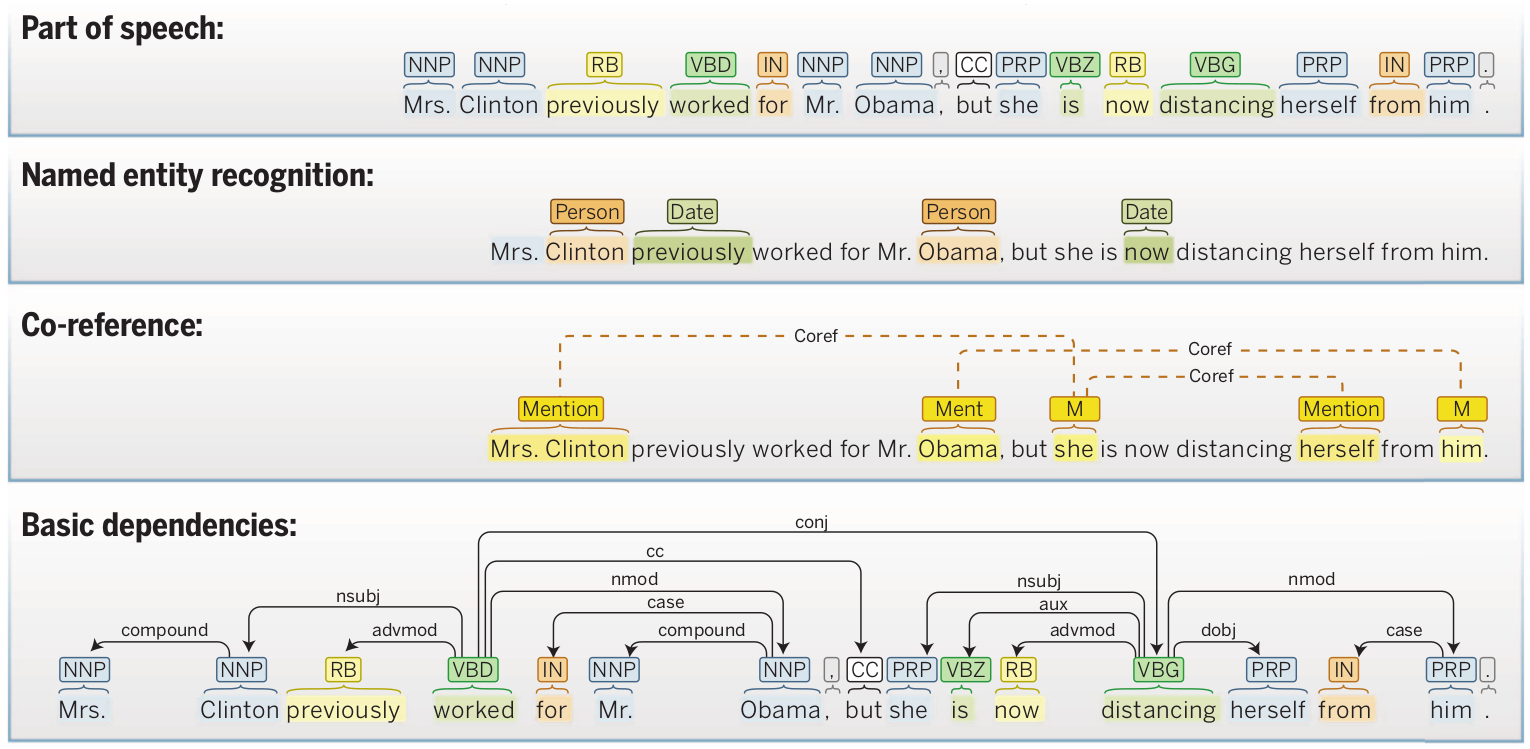
\includegraphics[width=1.5\textwidth]{gfx/corenlp}}
\caption[Ejemplo de parseo de dependencias 2]{Ejemplo de la salida del programa
  \textsc{CoreNLP}. De arriba a abajo, se muestra la categoría morfosintáctica
  de cada palabra, el nombre de algunas entidades, determina qué entidad hace
  co-referencia a la misma persona u organización y por último la estructura
  sintáctica de cada frase, usando un análisis de dependencias gramaticales.}
  \label{fig:corenlp}
\end{figure}

\section{Limitaciones}
\label{sec:nlplimits}

Aunque se han producido avances, una de las principales limitaciones del
\ac{NLP} hoy día es el hecho de que la mayoría de recursos y sistemas solo están
disponibles para los denominados \emph{\acp{HRL}}\graffito{\ac{HRL}: Idiomas de
  altos recursos}, estos lenguajes son el Inglés, Francés, Español, Alemán y
Chino. Por contra, hay una gran cantidad de \emph{\acp{LRL}}
--\graffito{\ac{LRL}: Idiomas de bajos recursos} como Bengalí, Indonesio,
Punjabí, Cebuano y Swahili -- hablados y escritos por millones de personas que
no disponen de este tipo de sistemas. Uno de los mayores retos para la comunidad
del lenguaje es desarrollar recursos y herramientas para cientos o miles de
lenguajes, no solo para unos pocos.

Aún existiendo bastante \emph{software} trabajando con \ac{NLP}, y para idiomas
\ac{HRL}, suelen obtenerse mejores resultados para un idioma en concreto, el
Inglés. Es por ello que este trabajo se ha centrado en desarrollar una fase del
\emph{pipeline} que se encuentra en todos los sistemas que realizan análisis de
sentimientos, y en general \ac{NLP} para el idioma Español. Como ejemplo podemos
citar el famoso \textsc{CoreNLP} \cite{Manning2014}.

En la \autoref{table:corenlpfeatures} se lista todo el \emph{pipeline} de
\textsc{CoreNLP} junto con el soporte para cada lenguaje. Como se aprecia, el
\emph{pipeline} esta completo únicamente para el Inglés. El objetivo de este
trabajo ha consistido en implementar un parseo de dependencias para el Español.

\definecolor{tick}{HTML}{5dc452}
\newcommand*{\checktikz}[1][]{\tikz[x=1em, y=1em]\fill[#1] (0,.35) -- (.25,0) --
  (1,.7) -- (.25,.15) -- cycle;}
\newcommand*{\ccheck}{\checktikz[tick,rounded corners=.5pt, draw=tick,
  thin]} %\checktikz[rounded corners=.5pt, draw=red, ultra thin]


\begin{table}[]
  \centering
  \caption{\emph{Pipeline} de \textsc{CoreNLP} y disponibilidad por lenguaje}
  \label{table:corenlpfeatures}
  \begin{tabular}{lllllll}
    \rowcolor[HTML]{443627} 
    \multicolumn{1}{c}{\cellcolor[HTML]{443627}{\color[HTML]{FFFFFF} \textbf{ANNOTATOR}}} & \multicolumn{1}{c}{\cellcolor[HTML]{443627}{\color[HTML]{FFFFFF} \textbf{AR}}} & \multicolumn{1}{c}{\cellcolor[HTML]{443627}{\color[HTML]{FFFFFF} \textbf{ZH}}} & \multicolumn{1}{c}{\cellcolor[HTML]{443627}{\color[HTML]{FFFFFF} \textbf{EN}}} & \multicolumn{1}{c}{\cellcolor[HTML]{443627}{\color[HTML]{FFFFFF} \textbf{FR}}} & \multicolumn{1}{c}{\cellcolor[HTML]{443627}{\color[HTML]{FFFFFF} \textbf{DE}}} & \multicolumn{1}{c}{\cellcolor[HTML]{443627}{\color[HTML]{FFFFFF} \textbf{ES}}} \\
    Tokenize / Segment & \ccheck & \ccheck & \ccheck & \ccheck &  & \ccheck \\
    Sentence Split & \ccheck & \ccheck & \ccheck & \ccheck & \ccheck & \ccheck \\
    Part of Speech & \ccheck & \ccheck & \ccheck & \ccheck & \ccheck & \ccheck \\
    Lemma &  &  & \ccheck &  &  &  \\
    Named Entities &  & \ccheck & \ccheck &  & \ccheck & \ccheck \\
    Constituency Parsing & \ccheck & \ccheck & \ccheck & \ccheck & \ccheck & \ccheck \\
    Dependency Parsing &  & \ccheck & \ccheck & \ccheck & \ccheck &  \\
    Sentiment Analysis &  &  & \ccheck &  &  &  \\
    Mention Detection &  & \ccheck & \ccheck &  &  &  \\
    Coreference &  & \ccheck & \ccheck &  &  &  \\
    Open IE &  &  & \ccheck &  &  & 
  \end{tabular}
\end{table}

Con la introducción del \emph{pipeline} de \textsc{CoreNLP}, se pasa ahora a
describir el proceso que todo sistema para \ac{NLP} debe seguir. Comenzaremos
mencionando un proceso genérico, para después profundizar en el \emph{pipeline}
de un \emph{software} especícifo, \textsc{CoreNLP} en nuestro caso.

\section{El pipeline genérico}
\label{sec:genericpipeline}

En esta sección se comentará el proceso habitual que suele seguirse como
\emph{pipeline} en los problemas de \ac{NLP}. Para ello se describirán los
distintos niveles de análisis en los que opera dicho \emph{pipeline}, así como
las diferentes aproximaciones que se usan y los problemas más comunes a los que
se enfrenta todo sistema que realice \ac{NLP}.

\citet{liu:2010} define una opinión como una quíntupla conteniendo el objetivo
de la opinión (o \emph{entidad}), el atributo del objetivo al que se dirige la
opinión, el sentimiento (o polaridad) de la opinión, pudiendo ser este positivo,
negativo o neutral, el poseedor de dicha opinión y la fecha en la que se
produjo. Formalmente se podría definir como la tupla:
\[
  (e_i, a_{ij}, s_{ijkl}, h_k, t_l)
\]
donde $e_i$ corresponde con el objetivo de la opinión i-ésima, $a_{ij}$ es el
j-ésimo atributo de $e_i$, $h_k$ el k-ésimo poseedor de la opinión, $t_l$
codifica el tiempo en el que se emitió la opinión y por último, $s_{ijkl}$ es la
polaridad de la opinión hacia el atributo $a_{ij}$ para la entidad $e_i$ por el
poseedor de la opinión $h_k$ en el momento $t_l$.

El principal objetivo del análisis de sentimientos consiste en encontrar todas
las tuplas $(e_i, a_{ij}, s_{ijkl}, h_k, t_l)$ en un documento o colección de
documentos.

\subsection{Pasos previos}
\label{subsec:previousSteps}

El procesamiento más usual para realizar tareas de análisis de sentimietos se
puede dividir en una serie de pasos definidos. Dichos pasos corresponden a la
adquisición del \emph{corpus} o datos, preprocesamiento del texto, el proceso
principal del análisis de sentimientos, agregación y resumen de los resultados y
por último, visualización. En los próximos apartados se mencionarán los tres
primeros.

\subsubsection{Adquisición de Datos}
\label{sec:dataacq}

En este paso se debe obtener el \emph{corpus} para el cual se desea realizar el
análisis de sentimientos. Actualmente existen dos aproximaciones para realizar
esta tarea. Una de ellas consiste en hacer uso de la \acfi{API}\acused{API} de
alguna página web de la que se desee extraer el \emph{corpus}. Una de las
\acp{API} más populares para este propósito es la de Twitter. La segunda
aproximación hace uso de \emph{Web Crawlers}\graffito{Rastreadores de Webs} para
extraer datos de las webs deseadas.

Ambas aproximaciones presentan sus ventajas y desventajas, y por tanto se debe
encontrar un equilibrio en función de cual se decida usar. Veamos algunos de
ellos.

Mediante el uso de una \ac{API} la implementación es sencilla, los datos
obtenidos están ordenados y poseen una estructura poco sujeta al cambio, sin
embargo, en función del proveedor de la \ac{API} se presentan ciertas
limitaciones. Siguiendo con Twitter, su \ac{API} limita a 180 consultas cada 15
minutos el número de peticiones que se pueden realizar. Además, su \ac{API} para
\emph{streaming} presenta otras limitaciones. En lugar de imponer límites a la
cantidad de peticiones, restringe el número de clientes que se pueden conectar
desde la misma dirección \textsc{ip} al mismo tiempo, así como la velocidad a la
que cada uno puede leer los datos. Pese a las limitaciones anteriores, la más
importante quizás sea que esta aproximación depende de la existencia de una
\ac{API} por parte del sitio web.

Por otro lado, la aproximación basada en rastreadores webs son bastante más
complejas de implementar, la razón principal se debe a que los datos obtenidos,
por norma general tendrán ruido y no estarán estructurados. Como beneficio, esta
aproximación tiene la capacidad no imponernos prácticamente ninguna
restricción. Si bien es cierto que se deben respetar ciertas normas y
protocolos, como las indicaciones del fichero
\textsc{robots.txt}\footnote{\url{http://www.robotstxt.org/robotstxt.html}} de
cada sitio web, no realizar múltiples peticiones al mismo servidor y espaciar
las mismas para no someter al servidor a demasiada carga.

\subsubsection{Preprocesamiento del texto}
\label{sec:textpreprocesing}

El segundo paso en el \emph{pipeline} del análisis de sentimientos es el
preprocesamiento del texto adquirido. En este paso se realizan varias tareas
habituales para el \ac{NLP} correspondientes al análisis léxico. Algunas de
estas tareas son:

\label{par:token}
\paragraph{Tokenización:}Es una técnica fundamental para la mayoría de tareas en
\ac{NLP}. Encargada de separar las cadenas de texto del documento completo en
una lista de palabras. Es muy sencilla de realizar para idiomas delimitados por
espacios como el Inglés, Español o Francés, pero se torna considerablemente más
compleja para idiomas donde las palabras no son delimitadas por espacios, como
el Japonés, Chino y Thai.

Los idiomas anteriores requieren de un proceso llamado segmentación de palabras,
el cual es un problema de etiquetado secuencial. Para resolverlo se usan
\acfi{CRF}\acused{CRF}, método que ha demostrado ser superior a los modelos de
Markov ocultos y modelos de Markov de máxima entropía \cite{Kudo04, tseng2005,
  Peng2004}. Debido a que es una técnica fundamental, existen multitud de
herramientas disponibles, para idiomas delimitados por espacios, el tokenizador
de Stanford\footnote{\url{http://nlp.stanford.edu/software/tokenizer.shtml}} o
el de
\textsc{OpenNLP}\footnote{\url{https://opennlp.apache.org/documentation/manual/opennlp.html\#tools.
    tokenizer}}. Para la segmentación de palabras en Chino, existen herramientas
como \textsc{ICTCLAS}\footnote{\url{http://ictclas.nlpir.org}},
\textsc{THULAC}\footnote{\url{http://thulac.thunlp.org}} y el segmentador de
Stanford\footnote{\url{http://nlp.stanford.edu/software/segmenter.shtml}}.

\paragraph{Stemming:}Proceso heurístico encargado de eliminar los afijos de la
palabra para dejarlos en su forma canónica (invariante, o raíz). Por ejemplo,
\emph{persona, personificar y personificación} pasan a ser \emph{persona} una
vez acabado este proceso.

\paragraph{Lematización:}Proceso algorítmico para convertir una palabra a su
forma de diccionario no-inflexible -- \emph{non-inflected} en inglés --. Esta
fase es análoga a la anterior (\emph{stemming}) pero se realiza a través de una
serie de pasos más rigurosos que incorporan un análisis morfológico de cada
palabra.

\paragraph{Eliminación de stopwords:} Actividad encargada de borrar las palabras
usadas para estructurar el lenguaje pero que no contribuyen de modo alguno a su
contenido. Algunos ejemplos de estas palabras pueden ser \emph{de, la, que, el,
  en, y, a, los, del, se, las, por, un, par, con}.\footnote{Para ver una lista
  completa de palabras visitar:
  \url{http://snowball.tartarus.org/algorithms/spanish/stop.txt}}

\paragraph{Segmentación de frases:}Procedimiento que separa párrafos en
sentencias. Presenta sus propios retos, ya que los signos de puntuación, como el
punto (.) se usan con frecuencia para marcar tanto el fin de una frase como para
denotar abreviaciones y números decimales.

\paragraph{POS tagging y parseo} o etiquetado morfosintáctico. Paso que etiqueta
cada palabra de una sentencia con su categoría morfosintática, como
\emph{adjetivo, nombre, verbo, adverbio} y \emph{preposición}. Estas etiquetas
pueden usarse como entrada para procesamientos futuros, como el parseo de
dependencias (Objetivo de este trabajo) o como característica para el proceso de
\ac{AA}. De igual manera que la segmentación, es un problema de etiquetado
secuencial. El etiquetado morfosintático proporciona información léxica, el
parseo obtiene información sintáctica. El parseo genera un árbol que representa
la estructura gramatical de una sentencia dada con la correspondiente relación
entre los distintos constituyentes. Este trabajo se ha centrado en construir un
parseo de dependencias para el Español.

Cabe destacar que no es obligatorio aplicar todos y cada uno de los pasos
anteriores. En función del tipo de aplicación se ejecutarán unos pasos u
otros. Por ejemplo, un sistema basado en \ac{AA} probablemente aplicará cada uno
de estos pasos con el fin de reducir la dimensionalidad y ruido del
problema. Por contra, una aproximación no-supervisada quizá necesite la
categoría sintáctica de algunas de las \emph{stopwords} para construir reglas de
dependencia con el fin de usarlas posteriormente en el proceso principal del
análisis. Es claro pues, que la aproximación no-supervisada en este caso deberá
omitir la fase eliminación de \emph{stopwords}. En \nameref{sec:approaches} se
describe con más detalle las diferencias entre aproximaciones supervisadas
frente a no supervisadas.

Por otra parte, existen otro tipo de pasos dependientes en su totalidad del
origen de los datos y el método de adquisición. En particular, los datos que se
obtengan a través de un rastreador web deberán ser procesados con fin de
eliminar las etiquetas \acfi{HTML}\acused{HTML} e información no textual -- como
imágenes y anuncios -- El texto extraido de Twitter necesitará de especial
atención en cuanto a \emph{hashtags}, menciones, \emph{retweets}, texto
póbremente escrito, emoticonos, carcajadas escritas y palabras con caráctares
repetidos --- \emph{siiiiiiiiiiii} ---

\subsection{Proceso principal del análisis de sentimientos}
\label{sec:omcore}

La tercera fase en el \emph{pipeline} es el proceso principal del análisis. A
continuación se mencionarán los distintos niveles de granularidad en los que
actuan las aproximaciones más comunes.

\subsubsection{Niveles de análisis}
\label{sec:anallevels}

Desde que el análisis de sentimientos comenzó a ganar popularidad, se han ido
proponiendo distintos niveles para el análisis en las distintas etapas. La
primera se realizaba a nivel del documento, donde el objetivo residía en
identificar la polaridad general del mismo. Más tarde, el interés se desplazó
hacia un nivel más específico, las setentencias. Por último, se bajó un paso más
en cuanto a la granularidad para interesarse a nivel de entidad. Cabe destacar
que los niveles más granulares pueden agruparse o conglomerarse para formar
niveles más altos -- menos granulares, a mayor escala -- Por ejemplo, una
análisis de sentimientos podría calcular la media de polaridades en una frase y
producir un resultado a nivel de sentencias. Veamos a continuación los distintos
niveles.

\paragraph{Nivel de documento:}A este nivel, el análisis trata de clasificar el
documento al completo con una polaridad positiva o negativa. La utilidad de este
nivel a menudo está limitada y por normal general se usa en el contexto del
análisis de reseñas \cite{Liu2012}. Formalmente, el objetivo para este tipo de
tareas puede definirse como una versión modificada de la representación
introducida en la \autoref{sec:genericpipeline} y corresponde a la búsqueda de
tuplas
\[
  (-, GENERAL, S_{GENERAL}, -, -)
\]
donde la entidad $e$, el poseedor de la opinión $h$, y el tiempo $t$ en el que
se manifestó la opinión se asumen conocidos o se ignoran. El atributo $a_j$ de
la entidad $e$ se corresponde con GENERAL. Todo esto implica que el análisis
devolverá sólamente la polaridad general del documento.\question{¿Pongo
  ejemplos? \emph{To give a few examples, in [47], Pang and Lee attempted to
    predict the polarity of movie reviews using three different machine learning
    techniques: Naïve Bayes, Maximum Entropy classification and Support Vector
    Machine (SVM). Similarly, in [50] the same authors tried to predict the
    rating of a movie given in a review, instead of just classifying the review
    into a positive or negative class.}}

\paragraph{Nivel de sentencia:} Análogo al anterior, ya que se podría considerar
una sentencia como un documento corto. Sin embargo, este nivel presenta algunos
pasos de preprocesamiento consistentes en separar el documento en oraciones,
paso que a su vez posee retos similares a la tokenización de idiomas no
delimitados por periodos --- visto en \nameref{par:token} ---

\paragraph{Nivel de entidad y aspecto:} El más granular de todos a los que el
análisis de sentimientos puede trabajar. A este nivel la tarea no consiste
únicamente en encontrar la polaridad de una opinión, también su objetivo --- a
quién va dirigida --- Por esto mismo, la definición de la quíntupla en la
\autoref{sec:genericpipeline} aplica al completo. El análisis a nivel de
documento y sentencias funcionan bien cuando el texto analizado contiene una
sola entidad y aspecto, pero empeoran para varios \cite{Feldman2013}. Para
resolver este tipo de problemas, algunos sistemas de análisis de sentimientos
basados en aspectos intentan detectar cada aspecto mencionado en el texto para
asociarlo con una opinión.

El primer trabajo que se ocupó de resolver este problema fue obra de
\citet{Hu2004}. \citeauthor{Hu2004} detectaban características de productos --
aspectos -- comentados con frecuencia por clientes, luego identificaban dichas
sentencias con opiniones, las evaluaban en base a su polaridad y finalmente
resumían los resultados.

\subsubsection{Otras aproximaciones}
\label{sec:approaches}

Existen dos aproximaciones para llevar a cabo el proceso de análisis de
sentimientos. Una basada en léxico, no supervisada. Esta aproximación depende
de reglas y heurísticas obtenidas del conocimiento lingüístico
\cite{VILARES2013}. La otra aproximación es supervisada, usa \ac{AA}, aquí se
utilizan algoritmos que aprenden la información subyacente de datos previamente
anotados, permitiendoles así clasificar instancias nuevas --- sin etiquetar
\cite{Pang:2002:TUS:1118693.1118704} ---. Aunque estas dos aproximaciones son las más usadas, existen
estudios que han demostrado buenos resultados al combinar ambas. Pasamos ahora a
describirlas en detalle.

\paragraph{Aproximación no supervisada basada en el léxico:} También llamada
basada en la semántica. Intenta determinar la polaridad del texto usando un
conjunto de reglas y heurísticas obtenidas del conocimiento del idioma. Los
pasos habituales consisten en marcar primero cada palabra y frase con su
correspondiente polaridad con ayuda de un diccionario. El siguiente paso
incorpora el análisis de modificadores de sentimientos -- como la negación -- y
su ámbito -- intensificadores y negación --. Por último se tratan las
conjunciones adversativas -- \emph{pero, aunque, mas} -- comprendiendo cómo
afectan a la polaridad y reflejándolo en la puntuación final del sentimiento
\cite{Liu2012}.

\question[inline]{Pongo ejemplos?}

\paragraph{Aproximación supervisada basada en aprendizaje:}Igualmente conocida
como aproximación basada en \ac{AA} o métodos estadísticos para la clasificación
de sentimientos. Consiste en algoritmos que aprenden los patrones subyacentes de
los datos de entrenamiento --- datos cuya clase o etiqueta se conoce para cada
instancia --- para después intentar clasificar nuevos datos suministrados al
algoritmo, esta vez sin estar etiquetados. Los pasos a seguir en una
aproximación de este tipo consisten en realizar algo de ingeniería de
características que respresenten el objeto cuya clase se quiere predecir. Tras
esto, se usan dichas representaciones como como entrada del algoritmo. Algunas
de las características más usadas en al análisis de sentimientos son: frecuencia
del término, categorías morfosintáctica -- \ac{POS} \emph{tags} -- palabras y
frases con sentimientos, reglas de opinión,  modificadores del sentimiento y
dependencias sintácticas, por mencionar algunas \cite{Liu2012}.

\question[inline]{De nuevo, pongo ejemplos?}

\paragraph{Aproximación basada en conceptos:}Relativamente moderna. Consiste en
usar \emph{ontologías}\graffito{Una ontología se define como un modelo que
  conceptualiza el conocimiento de un dominio dado, de tal forma que pueda ser
  comprendido tanto por humanos como máquinas.} para apoyar la tarea del
análisis de sentimientos. Las ontologías suelen presentarse como gráfos donde
los conceptos se asocian a nodos enlazados por relaciones. El estudio realizado
por \citet{Zhou2007} analiza en profundidad las ontologías, así como sus
aplicaciones y desarrollo.

Una de las ventajas de usar métodos no supervisados reside en la no dependencia
de grandes cantidades de datos para entrenar a los algoritmos. Aún así, sigue
siendo necesaria la construcción u obtención de un léxico para los
sentimientos. Los métodos no supervisados son menos dependientes del dominio que
los métodos supervisados. De hecho, los clasificadores entrenados en un dominio
específico muestran de forma consistente peor comportamiento cuando son
ejecutados en otros dominios \cite{anthony2005}.


\section{El pipeline de \textsc{CoreNLP}}
\label{sec:corenlppipeline}

En la \autoref{sec:genericpipeline} se ha visto el proceso genérico a seguir
para problemas de \ac{NLP}, se presenta ahora una breve descripción de
los pasos que se mostraron en la \autoref{table:corenlpfeatures},
correspondientes al \emph{pipeline} para un software concreto ---
\textsc{CoreNLP} \cite{Manning2014} --- Como se aprecia, dicho \emph{pipeline}
solo está totalmente completo para el Inglés.

\textsc{CoreNLP} viene empaquetado con los modelos para Inglés. Es posible
descargar modelos para distintos idiomas, pero por separado. El soporte para
estos idiomas no es completo. Los pasos del \emph{pipeline} mencionados a
continuación se centran en la versión para el Inglés. En
\nameref{sec:approaches} se citaron los distintos modos de realizar tareas para
\ac{NLP}, los modelos de \textsc{CoreNLP} entrenan modelos usando tanto métodos
de \ac{AA} supervisados como basándose en reglas.

\paragraph{Tokenizador:} \emph{Tokeniza} el texto en secuencias de símbolos. El
componente para el Inglés proporciona un \emph{tokenizador} al estilo
\acfi{PTB}\acused{PTB} que ha sido ampliado para tratar con texto de la web y
con ruido. Los componentes correspondientes para el Chino y Árabe proporcionan
segmentación de palabras y \emph{clitic}. Como proceso final, el
\emph{tokenizador} almacena los desplazamientos de caracteres de cada símbolo en
el texto de entrada.

\paragraph{CleanXML:} Elimina las etiquetas \acfi{XML} del documento.

\paragraph{Ssplit:} Separa una secuencia de símbolos en frases.

\paragraph{Truecase:} Determina la probabilidad de un símbolo de estar en
mayúscula en el texto --- es decir, la probabilidad de que, en un texto bien
escrito, dicho símbolo debiera estar en mayúscula. --- cuando esta información
no está disponible, \eg~ un texto con todas las letras en mayúsculas. Este
proceso se implementa con un modelo discriminativo usando un etiquetador de
secuencias \ac{CRF} \cite{Finkel2005}.

\paragraph{Pos:} Etiqueta símbolos con su correspondiente categoría
morfosintática -- \ac{POS} \emph{tag} -- haciendo uso de un etiquetador de
máxima entropía \cite{Toutanova2003}.

\paragraph{Lemma:} Genera la raíz -- o \emph{lemma} -- para todos los símbolos
en la anotación.

\paragraph{Gender:} Añade información sobre el género más probable a los
nombres.

\paragraph{Ner:} Reconoce nombres --- \textsc{Persona, Lugar, Organización,
  Miscelánea} --- y entidades numéricas --- \textsc{Dinero, Número, Fecha, Hora,
  Duración}. --- En los etiquetados por defecto, las entidades para nombres se
reconocen mediante una combinación de secuencias de \acp{CRF} entrenados en
varios \emph{corpus} \cite{Finkel2005}. Las entidades numéricas son reconocidas
usando dos sistemas basados en reglas, uno para el dinero y números, y otro
sistema \emph{estado del arte} para procesar expresiones temporales
\cite{Chang2012}.

\paragraph{Regexner:} Implementa un \textsc{Ner} simple basado en reglas usando
secuencias de símbolos mediante expresiones regulares. El objetivo de este paso
del \emph{pipeline} es proporcionar un \emph{framework} que permita al usuario
incorporar etiquetas \textsc{NE} que no están anotadas en \emph{corpus}
\textsc{NL} tradicionales. Por ejemplo, la lista por defecto de expresiones
regulares distribuida en los modelos de \textsc{CoreNLP} reconoce ideologías,
nacionalidades, religiones y títulos.

\paragraph{Parse:} Proporciona un análisis sintáctico completo, incluyendo
representaciones tanto de dependencias como constituyentes. Está basado en un
parseador probabilístico \cite{Klein2002, deMarneffe2008}.

\paragraph{Sentiment:} Análisis de sentimientos con un modelo compositivo sobre
árboles usando \emph{deep learning} \cite{socher2013}. La puntuación asignada a
un sentimiento se calcula mediante los nodos de un árbol binario para cada
sentencia, incluyendo, en particular, el nodo raíz de cada frase.

\paragraph{Dcoref:} Detecta menciones y resolución de coreferencias tanto pronominales como
nominales \cite{Lee2013}. Se devuelve el grafo de coreferencia del texto al
completo, con las palabras principales de las menciones como nodos.

En la \autoref{fig:corenlppipe} se muestra el \emph{pipeline} completo de \textsc{CoreNLP}.

\begin{figure}[bth]
  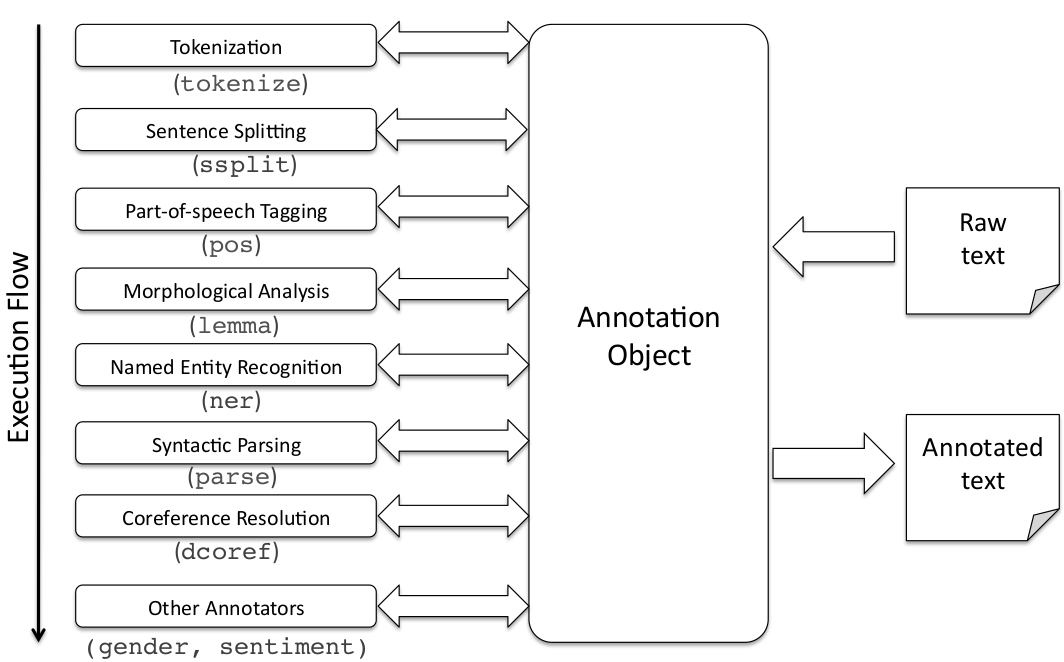
\includegraphics[width=1\linewidth]{gfx/corenlppipe.png}
  \caption[Visualización del \emph{pipeline} de \textsc{CoreNLP}]{Visión general
    de la arquitectura. El texto a procesar se añade a un objeto
    \textsc{Annotation}. Posteriormente una secuencia de etiquetadores añaden
    información sobre qué fases del \emph{pipeline} deben ejecutarse. El
    resultado contiene el texto procesado, puede obtener en formato \ac{XML} o
    texto plano.}
  \label{fig:corenlppipe}
\end{figure}

\section{Software Existente}
\label{sec:nlpsoftware}

\myTodo[inline]{Menciono software existente?}

\section{Estado del arte}\myTodo[fancyline]{Leer state-of-the-art de
  1-s2.0-S1566253515000536-main y 1-s2.0-S1566253516301117}
\label{sec:stateoftheart}

